\documentclass{article}

% Camera-ready, Evaluations and Datasets Track (accepted, poster).
% [final] de-anonymises and prints the track notice; [eandd] names the track.
\usepackage[final,eandd]{neurips_2026}

\usepackage[utf8]{inputenc}
\usepackage[T1]{fontenc}
\usepackage{hyperref}
\usepackage{url}
\usepackage{booktabs}
\usepackage{amsfonts}
\usepackage{amsmath}
\usepackage{amssymb}
\usepackage{nicefrac}
\usepackage{microtype}
\usepackage{xcolor}
\usepackage{graphicx}

\DeclareMathOperator*{\argmax}{arg\,max}

\newcommand{\dataset}{\textsc{CTSpinoPelvic1K}}
\newcommand{\TS}{TotalSegmentator}
\newcommand{\SOTA}{TotalSegmentator}
\newcommand{\sota}{TS}
\newcommand{\VERIDAH}{VERIDAH}
\newcommand{\VerSe}{VerSe}

% Patrick Schwing's affiliation is not recorded anywhere in the project
% files; it must be confirmed by the corresponding author before upload.
\newcommand{\PatrickAffil}{\textcolor{red}{[Affiliation to be confirmed]}}

\title{Not All Spines Are Created Equal:\\
How CT Segmenters Fail on Lumbosacral Transitional Vertebrae}

\author{%
  Gregory John Schwing\thanks{Corresponding author:
    \texttt{gregory.schwing@med.wayne.edu}.} \\
  Department of Surgery \\
  Detroit Medical Center and Wayne State University \\
  Detroit, Michigan, USA \\
  \And
  Patrick Schwing \\
  \PatrickAffil{} \\
  \And
  Miraziz Ismoilov \\
  Department of Radiology \\
  Detroit Medical Center and Wayne State University \\
  Detroit, Michigan, USA \\
  \AND
  Nizar Alnabahneh \\
  Department of Radiology \\
  Detroit Medical Center and Wayne State University \\
  Detroit, Michigan, USA \\
  \And
  Loren Schwiebert \\
  Department of Computer Science \\
  Wayne State University \\
  Detroit, Michigan, USA \\
}

\begin{document}

\maketitle

% ============================================================================
\begin{abstract}
Wrong-level spine surgery remains a persistent
never-event, and the lumbosacral transitional vertebra
(LSTV, 5--35\% prevalence) is its largest anatomic
driver. We audit \TS{}---the most widely deployed CT
segmentation system and default back-end of
3D~Slicer---and show that on lumbarization cases its
output reproduces the pattern of a one-level miscount:
lacking an L6 class, it shifts lumbar labels caudally by
one level, and junction-DSC drops 29 points on Any-LSTV
($0.824 \to 0.534$; $n{=}7$ cases with a scorable
junction). No existing CT benchmark surfaces this---not
\TS{}'s own evaluation, not \citet{Li2025LumbarMechanism}
(the per-class DSC frontier on the matched COLONOG split),
and not \VERIDAH{} (vertebra-\emph{labeling} SOTA on a
private cohort, on pre-localized crops with no pelvis).
We contribute: (i)~an LSTV-stratified evaluation protocol
(per-class DSC, junction-DSC over a 40\,mm L5/S1 window,
per-class voxel confusion at the junction) that measures
the level shift and frames it as a plausible automated
wrong-level-risk mechanism; (ii)~\dataset{}---1{,}153 CT
records across 802 patients with unified spinopelvic
masks, 33 LSTV-positive patients in a six-way phenotype
taxonomy derived from the source annotations' filenames
and lumbar counts, and Castellvi typing (I--IV) of all 33
by two radiology residents ($\kappa{=}0.74$);
(iii)~the first publicly released merge-based
dual-spinopelvic CT segmenter, exceeding \TS{} on sacrum
($0.817 \to 0.969$) with released weights; (iv)~a
same-data, same-fold unmerged control with an explicit L6
class that still labels most ground-truth L6 voxels L5,
isolating the training-side L5/L6 merge as the component
that removes the collision, while a residual
L4/last\_lumbar collision on count-style sacralization
motivates a downstream sequence predictor. Only 7 LSTV
cases fall in the held-out split; every stratified number
is reported with its $n$.
\end{abstract}

% ============================================================================
\section{Introduction}
\label{sec:intro}

Wrong-level spine surgery is a persistent never-event in
operative spine
care~\citep{Konin2010LumbosacralRelevance}. Despite
intraoperative imaging and surgical-pause checklists, the
most common cause---failure to correctly count vertebral
levels in the presence of an LSTV---continues to account for
the majority of reported wrong-level lumbar
incidents~\citep{Carrino2011EffectImaging}. The mechanism is
well documented: a surgeon counts lumbar bodies upward from
the sacrum, finds five (because lumbarization presents a
sixth lumbar body that has not been recognized), and labels
the bottom body as L5 when it is anatomically L6. Surgery
proceeds one level caudal to the intended target.

Modern radiology workflows increasingly route automated
segmentation as an upstream substrate for clinical
decision-making. The most widely deployed CT segmentation
system in this role is
\TS{}~\citep{Wasserthal2023TotalSegmentator:Images}: an
nnU-Net trained on 1{,}204 routine CTs to delineate 104
anatomic structures, the default segmentation back-end of
3D~Slicer, with thousands of clinical and research
installations. The original paper reports an aggregate
test-set Dice of 0.943 across all 104 classes and
qualitatively documents two spine failure modes
affecting neighboring-vertebrae label confusion (1\%
of cases) and neighboring-rib confusion (12\%). \TS{} is neither the
only public CT spine segmenter nor the per-class DSC
frontier on the matched CTSpine1K~+~CTPelvic1K (COLONOG)
split (\S\ref{sec:related}); it is, however, the model
surgeons and downstream tools consume. This paper
concerns one anatomic class on which \TS{} does not
perform at its headline level, and the consequences
when it does not.

\paragraph{The risk mechanism.}
On lumbarized spines, \SOTA{} produces an output pattern
that matches the mechanism of the surgical miscount. Its
label vocabulary contains L1--L5 but no L6 class. On a
lumbarized spine (six lumbar bodies plus sacrum), the model
distributes its five lumbar labels across the six bodies by
shifting caudally by one anatomic level: the body that is
anatomically L6 receives the L5 label, the body that is
anatomically L5 receives the L4 label, and so on. A plan
that took the disc between predicted-L4 and predicted-L5
as L4--L5 would land on the anatomical L5--L6 disc. We
present this as a \emph{plausible automated
wrong-level-risk mechanism}: the paper measures how often
the shifted output occurs and what it looks like at the
junction. It does not evaluate surgical-planning software,
reader behaviour or downstream workflow, and no
wrong-level event is attributed to a segmenter here.

\paragraph{The architectural alternative: \VERIDAH{}.}
\citet{Moller2026VERIDAH:Sequences} label transitional
vertebrae with a per-vertebra classifier trained with
L5/L6 merged, followed by a constrained sequence predictor
that restores the count (\S\ref{sec:related}). Whether a
voxel-wise network trained at full resolution with the same
merge needs the sequence predictor at all has never been
tested; we supply that test.

\paragraph{The evaluation gap.}
Neither \SOTA{}, \VerSe{}~\citep{Sekuboyina2021VerSe:Images},
CTSpine1K~\citep{Deng2021CTSpine1K:Tomography}, nor
CTPelvic1K~\citep{Liu2021DeepModels} report LSTV-stratified
performance; earlier CT labelers excluded the failure
mode~\citep{Sekuboyina2020LabelingAnatomy}, and \VERIDAH{}
reports anomaly performance on a private cohort. A
production model therefore emits a confident, locally
well-formed, caudally-shifted prediction on a
5--35\%-prevalence variant with no error signal at
evaluation time. Closing the gap requires hardware:
fitting lumbar spine and pelvis at
$0.75{\times}0.75{\times}0.80$\,mm and a
$256{\times}320{\times}320$ patch consumes ${\sim}100$\,GB
of GPU memory, available on an H200 but not on the
L40S/A100/H100 GPUs that bracket \SOTA{}'s training
configuration.

\paragraph{Contributions.}
\begin{enumerate}
\item[(i)] \textbf{The level shift in \sota{},
  quantified.} An LSTV-stratified evaluation protocol
  (per-class DSC, junction-DSC over a 40\,mm L5/S1
  window, per-class voxel confusion at the junction)
  measures \sota{}'s systematic one-level caudal shift
  on lumbarization (L4=0.388, L5=0.291 over 14 patients;
  95\%+ of GT-L6 voxels labeled L5 on the case study,
  \S\ref{sec:case_study}) and the structural absence of
  L6 across all evaluation cases, and frames the shift
  as a plausible automated wrong-level-risk mechanism.
\item[(ii)] \textbf{\dataset{}: a stratified spinopelvic
  benchmark.} 1{,}153 abdominal CT records across 802
  patients, unified spinopelvic masks, 33 LSTV-positive
  patients in a six-way subtype taxonomy
  (lumb $n{=}14$; sacr\_count $n{=}9$; full sacralization
  $n{=}6$; semi-sacralization $n{=}2$; ambiguous $n{=}2$),
  and a registration-free fusion pipeline that resolves a
  previously undocumented Y-axis coordinate-convention
  mismatch between CTSpine1K and CTPelvic1K. The subtypes
  come from the source annotations (filename qualifiers
  and lumbar counts), not from image reads; the Castellvi
  layer (I--IV, all 33) is a two-resident read with
  $\kappa{=}0.74$ and no senior adjudication
  (\S\ref{sec:castellvi}). Both source datasets share
  the COLONOG cohort that underlies \VerSe{} and
  CTSpine1K, but neither encodes pelvic context with LSTV
  stratification.
\item[(iii)] \textbf{First publicly released merge-based
  LSTV-handling dual-spinopelvic CT segmenter.} A 5-fold CV nnU-Net
  3d\_fullres baseline on H200 hardware adopting
  \VERIDAH{}'s training-side merge
  (last\_lumbar = L5+L6) at the voxel level, with
  pelvic-class supervision in a single forward pass.
  We exceed \sota{} on sacrum and uniquely deliver both
  spine and pelvis with released weights
  (Table~\ref{tab:comparison}); \S\ref{sec:related}
  details the reproducibility tiers separating
  openly-released from paper-only baselines.
\item[(iv)] \textbf{Empirical isolation: the merge is
  necessary and insufficient.} A same-data, same-fold,
  same-architecture control trained \emph{without} the
  merge, with an explicit L6 class and L6 oversampling,
  still labels most GT-L6 voxels L5
  (\S\ref{sec:unmerged}), so the merge---not the added
  data or the added class---removes the L5/L6 collision
  driving \sota{}'s level shift. The merge in turn exposes
  a residual L4/last\_lumbar collision on count-style
  sacralization, isolating the component of \VERIDAH{}'s
  success attributable to its sequence predictor---a
  direction \VERIDAH{}'s authors could not ablate.
\end{enumerate}

% ============================================================================
\section{Related Work}
\label{sec:related}

\paragraph{Wrong-level spine surgery and LSTV.}
\citep{Konin2010LumbosacralRelevance,Carrino2011EffectImaging,Sekharappa2014LumbosacralSignificance}
document LSTV-induced miscounting (5--35\% prevalence) without
addressing automated segmentation as a miscount-propagation
pathway. \citet{Kwak2025AutomatedModel} detect LSTV on plain
radiographs (binary; different modality).

\paragraph{Production CT spine and pelvic segmentation.}
\TS{}~\citep{Wasserthal2023TotalSegmentator:Images}, an nnU-Net
trained on 1{,}204 CTs and the default 3D~Slicer back-end,
has no L6 class and no LSTV stratification; we audit it as
the production system downstream pipelines actually consume,
not as a per-class DSC frontier.
\citet{Li2025LumbarMechanism} hold the published per-class
DSC frontier on a COLONOG split (731 scans; 440/146/145)
but release neither weights nor code (paper-only) and do
not stratify by LSTV. \citet{Liu2025AutomaticDataset}
release FracSegNet (PENGWIN+CTPelvic1K), a pelvic-only
cascaded 3D nnU-Net providing sacrum and L/R hipbone; their
qualitative note of sacralization degradation (their
\S4.3) corroborates the LSTV gap our benchmark surfaces.
Table~\ref{tab:comparison} compares all baselines.

\paragraph{Vertebra-labeling SOTA: \VERIDAH{}.}
\citet{Moller2026VERIDAH:Sequences} address transitional-vertebra
\emph{labeling} (distinct from segmentation): a four-head
3D DenseNet169 classifier on per-vertebra crops, trained
with L5/L6 (and T12/T13) merged, plus a constrained
sequence predictor enforcing 4--6 lumbar bodies (terminal
double-L5 encodes L6). On a private CT cohort of 1{,}536
volumes \VERIDAH{} reports 99.18\% subject-level perfect
labeling versus prior CT SOTA~\citep{Meng2023VertebraeCycle}
77.81\%. It requires upstream centroids (\VerSe{}-derived
models or SPINEPS~\citep{Moller2024SPINEPSautomaticSegmentation}),
excludes the pelvis, and validates privately. Its ablation
(Table~5) shows the sequence predictor adds substantial
value, but the comparison against direct semantic
segmentation on a public LSTV-stratified split is
missing---the gap our baseline (\S\ref{sec:baseline}) fills.

\paragraph{Benchmarks and evaluation rigor.}
\VerSe{}~\citep{Sekuboyina2021VerSe:Images} (460 CT volumes)
is the only public CT benchmark whose label vocabulary
includes L6 (label~25) but it is unstratified by LSTV and
lacks pelvic GT; earlier CT labelers explicitly excluded
the failure mode~\citep{Sekuboyina2020LabelingAnatomy}.
Stratified safety-critical
reporting~\citep{Maier-Hein2024MetricsValidation}
motivates~\S\ref{sec:protocol}.

% ============================================================================
\section{Failure-Mode Analysis: \sota{} on LSTV}
\label{sec:audit}

We evaluate \SOTA{} v2 (\texttt{total} task) zero-shot at
full resolution on the full \dataset{} matched cohort.
\SOTA{} was not trained on any \dataset{} case, so every
case is valid; this provides 1{,}152 of \dataset{}'s
1{,}153 records (one record dropped due to \sota{}
inference failure) aggregated to 801 patients via
patient-level merging, including 33 LSTV-positive
patients. Full-resolution mode isolates the failure as a
property of label vocabulary and training distribution
rather than inference resolution.

Table~\ref{tab:sota_stratified} reports performance by
phenotype. On normal anatomy ($n{=}768$) \SOTA{} performs at
its published level. On Any-LSTV ($n{=}33$) every lumbar
metric drops; lumbarization collapses caudally
(L1=0.878\,$\to$\,L4=0.388\,$\to$\,L5=0.291 over 14
patients). Junction-DSC is scorable only where the ground
truth holds both L5 and sacrum: 334 normal patients and 7
LSTV patients (3 lumbarization: 0.22, 0.23, 0.62; 2
count-style sacralization: 0.47, 0.93; 2 full
sacralization: 0.43, 0.84), so the 29-point Any-LSTV drop
in the abstract rests on 7 patients. Per patient, L5 DSC
falls below 0.5 in 10 of 14 lumbarization cases (Wilson
95\% interval 45--88\%) and in 9 of 9 count-style
sacralization cases (70--100\%), against 9 of 750 normal
cases (0.6--2.3\%). \textsc{L6} predictions are
structurally zero across all 1{,}152 records (0--0.3\%).

\begin{table}[t]
\caption{\sota{} zero-shot stratified by LSTV phenotype on
\dataset{}, full-resolution mode; $n$ is patients.
Junction DSC over a 40\,mm L5/S1 axial window is scorable
only where GT holds L5 and sacrum ($n_\text{jxn}$).
$\dagger$: no record with a scorable junction.}
\label{tab:sota_stratified}
\centering
\small
\resizebox{\linewidth}{!}{%
\begin{tabular}{lrcccccccrr}
\toprule
\bfseries Subgroup & \bfseries $n$ &
\bfseries L1 & \bfseries L2 & \bfseries L3 & \bfseries L4 & \bfseries L5 &
\bfseries Sac & \bfseries Hips &
\bfseries Jxn DSC & \bfseries $n_\text{jxn}$ \\
\midrule
All cases                              & 801 & 0.911 & 0.906 & 0.913 & 0.914 & 0.913 & 0.817 & 0.929 & 0.818 & 341 \\
Normal                                 & 768 & 0.921 & 0.918 & 0.929 & 0.936 & 0.938 & 0.817 & 0.929 & 0.824 & 334 \\
\midrule
Any LSTV                               & 33  & 0.681 & 0.615 & 0.523 & 0.367 & 0.314 & 0.822 & 0.929 & 0.534 & 7 \\
\quad Lumbarization                    & 14  & 0.878 & 0.853 & 0.690 & 0.388 & 0.291 & 0.833 & 0.928 & \textbf{0.357} & 3 \\
\quad Sacralization (count-style)      &  9  & 0.265 & 0.100 & 0.055 & 0.001 & 0.000 & 0.814 & 0.926 & 0.697 & 2 \\
\quad Semi-sacralization               &  2  & 0.951 & 0.951 & 0.951 & 0.955 & 0.956 & 0.824 & 0.937 & $\dagger$ & 0 \\
\quad Sacralization (full)             &  6  & 0.718 & 0.676 & 0.673 & 0.724 & 0.793 & 0.826 & 0.932 & 0.636 & 2 \\
\quad Ambiguous                        &  2  & 0.952 & 0.951 & 0.882 & 0.678 & 0.374 & 0.771 & 0.932 & $\dagger$ & 0 \\
\midrule
\textsc{L6 emit}                       &     &       &       &       &       &       &       &       & \multicolumn{2}{r}{0 / 1152} \\
\bottomrule
\end{tabular}%
}
\end{table}

\paragraph{The level-shift mechanism.}
The asymmetry between lumbarization (severe, caudally
progressive) and count-style sacralization (uniform
collapse) follows from a single fact: \SOTA{}'s output head
has no L6 class. For 6-vertebra anatomies the model
compresses 6 anatomic units into 5 labels by shifting label
assignment caudally; the most rostral body remains L1
(escape into thoracic vertebrae), but every successive body
is misaligned, with the final body labeled L5 when it is
anatomically L6. For 4-vertebra anatomies the model emits
standard L1--L5, overshooting the GT lumbar count and
producing a $+1$-level offset uniformly. The level-shift
mechanism is the segmentation analog of the surgical
miscount~\citep{Konin2010LumbosacralRelevance}.

% ============================================================================
\section{Case Study: the Level Shift at the Junction}
\label{sec:case_study}

Aggregate metrics establish the population pattern; the
case study establishes the mechanism at the level a
surgeon would consume the output. Token~215 is a
lumbarization case (six lumbar bodies; Castellvi Ib by
consensus, one of the six cases the two readers graded
differently, \S\ref{sec:castellvi}). Table~\ref{tab:case215}
reports per-class DSC: L1 and L2 are well-placed ($0.954$,
$0.927$), L3 is partially correct ($0.594$), and
\textbf{L4, L5, and L6 all collapse to dice~zero}---no
GT-L4 or GT-L5 voxel correctly labeled and no L6 voxel
emitted. The pelvic classes remain at near-Normal accuracy:
the failure is local to the lumbosacral count, not a
general degradation of \sota{} on this patient.

\begin{table}[h]
\caption{Token~215 (lumbarization, 6 lumbar bodies):
per-class \sota{} zero-shot DSC. L4, L5 and L6 collapse to
zero because \sota{} compresses 6 bodies into 5 labels;
pelvic classes are unaffected. $\dagger$~\sota{} has no L6
label.}
\label{tab:case215}
\centering
\small
\begin{tabular}{lccccccccc}
\toprule
\bfseries Class & L1 & L2 & L3 & L4 & L5 & L6 & Sacrum & Hip$_L$ & Hip$_R$ \\
\midrule
\bfseries DSC & 0.954 & 0.927 & 0.594 & \textbf{0.000} & \textbf{0.000} & \textbf{0.000}$^{\dagger}$ & 0.817 & 0.922 & 0.926 \\
\bottomrule
\end{tabular}
\end{table}

\begin{figure}[h]
\centering
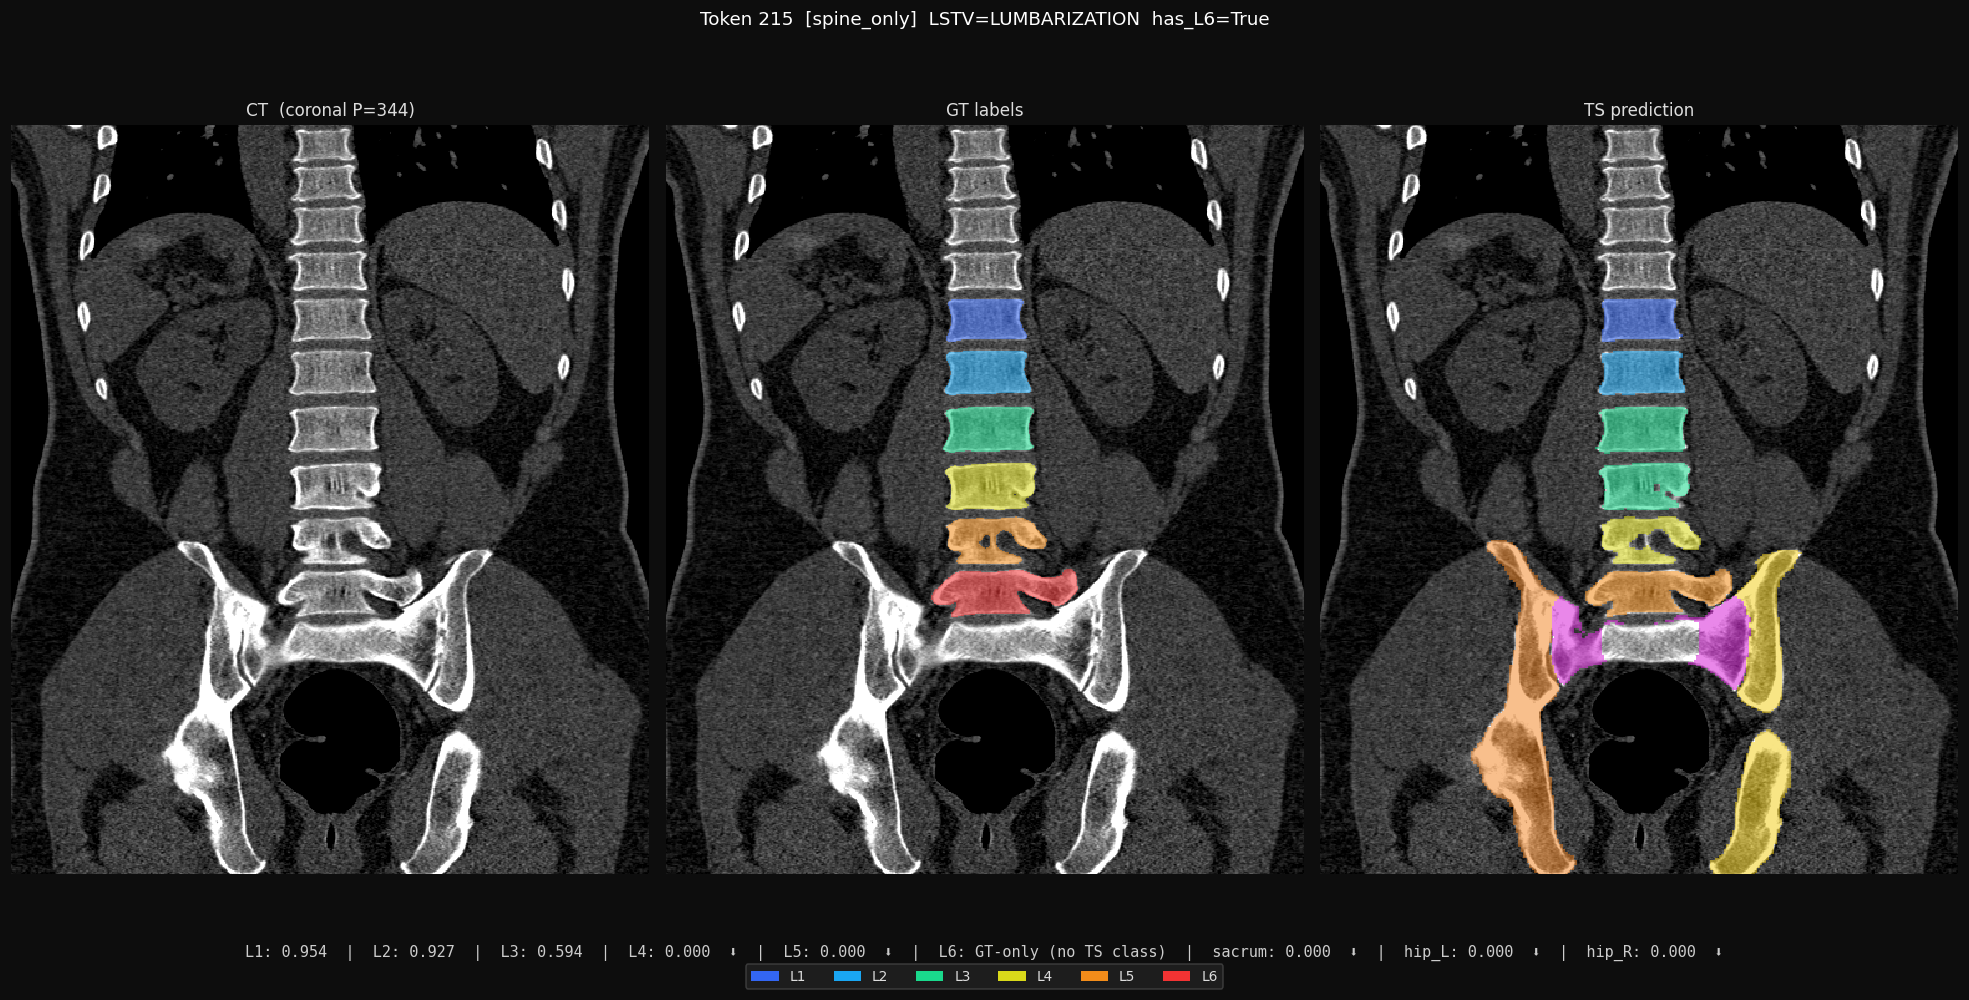
\includegraphics[width=\linewidth]{figs/lstv_lumbarization_215_spine_only.png}
\caption{Token~215, lumbarization (6 lumbar bodies): \sota{}
predictions on CT. Predicted-L3 absorbs anatomical L3 and
L4, predicted-L4 sits on anatomical L5, predicted-L5 on
anatomical L6, which has no label in \sota{}'s output head.
Five compact, well-formed predictions, every label below
L2 one level off. Quantified in Table~\ref{tab:case215}.}
\label{fig:case215}
\end{figure}

\paragraph{Why the pattern matters.}
A reader who took the segmentation at face value and
targeted the disc between predicted-L4 (anatomical L5) and
predicted-L5 (anatomical L6) would be one level caudal to
an L4--L5 intent. The output is locally well-formed: five
compact vertebral predictions in roughly correct positions,
detectable only by counting bodies (six lumbar, not five),
which downstream pipelines do not perform. Whether a
surgeon or a planning tool would in fact act on such an
output is not tested here; the claim is the mechanism and
its frequency, not a measured clinical harm.

% ============================================================================
\section{\dataset{}: Construction and Composition}
\label{sec:dataset}

\dataset{} fuses CT scans from
COLONOG~\citep{Smith2015DataCOLONOGRAPHY} with annotations
from CTSpine1K~\citep{Deng2021CTSpine1K:Tomography}
(\VerSe{}-derived per-vertebra masks) and
CTPelvic1K~\citep{Liu2021DeepModels} (sacrum and bilateral
hips). The same COLONOG cohort underlies \VerSe{} and
CTSpine1K; \dataset{}'s contribution is the patient-level
fusion of CTSpine1K's vertebra masks with CTPelvic1K's
pelvic masks plus the LSTV-stratification overlay neither
source provides. Of 1{,}153 matched records, 342 carry
fused (spine + pelvis) ground truth, 352 are separate-mode,
90 are spine-only, and 20 are pelvic-only
(Table~\ref{tab:scan_stats}).

\paragraph{Release used.}
Every number in this paper was computed on the April 2026
release (the HuggingFace export finalized 25 April 2026,
later labelled v1 in the repository; training began 3 May
2026): 1{,}153 records across 802 patients, a ten-class
scheme (background, L1--L6, sacrum, left and right hip)
merged to nine classes for training, and separate
spine-only and pelvic-only records for patients whose two
source annotations lie on different acquisitions. The
archive of record is the Zenodo concept DOI
\href{https://doi.org/10.5281/zenodo.22139642}{10.5281/zenodo.22139642},
whose current version is v11
(\href{https://doi.org/10.5281/zenodo.22797014}{10.5281/zenodo.22797014},
18 September 2026). v11 differs from the April release as
follows: one record per patient (802 records), each
separate-mode patient's missing pelvis completed on the
spine's series by out-of-fold pseudolabelling; VerSe-native
identifiers (L1--L6 = 20--25, sacrum 26, hips 30/31) with
femora, per-level ribs, lumbar ribs and surgical hardware
added as further classes; hip-laterality corrections on 22
records and hand corrections on five; both Castellvi reads
and their consensus in the manifest; and the CT images
supplied by TCIA series crosswalk and rebuild script, with
a HuggingFace mirror carrying the volumes. The 802 patients
and the 33 Castellvi-graded patients are the same in both.
Nothing here was recomputed on v11.

\begin{table}[t]
\caption{\dataset{} composition; LSTV phenotype
breakdown and split counts in Table~\ref{tab:castellvi_dist}.}
\label{tab:scan_stats}
\centering
\small
\begin{tabular}{lcc}
\toprule
\bfseries Property & \bfseries Value & \bfseries LSTV cases \\
\midrule
Patients matched (\dataset{})           & 802     & --- \\
Records matched (\dataset{})            & 1{,}153 & 33 patients (44 records) \\
\quad Fused (spine + pelvis)            & 342     & --- \\
\quad Separate (spine + pelvic)         & 352     & --- \\
\quad Spine-only / Pelvic-only          & 90 / 20 & --- \\
\bottomrule
\end{tabular}
\end{table}

\paragraph{Patient-anchored fusion and coordinate
correction.} Patient identity is resolved via canonical UID
matching (825/825 patients). Each mask is assigned to its
source CT acquisition by intra-patient bone-HU
maximization,
$s^*(m) = \argmax_{s \in \mathcal{S}_p}
|\{v \in \mathcal{L}(m, s) : I_s(v) > 200\,\text{HU}\}|/|\mathcal{L}(m, s)|$,
a metadata-free oracle since \texttt{SeriesDescription}
fields are unreliable in TCIA releases (99.6\% spine,
100\% pelvic placement). CTSpine1K and CTPelvic1K were
converted from DICOM with different \texttt{dcm2niix}
invocations, producing a systematic Y-axis sign reflection
in NIfTI affines; we detect via affine-derived center sign
and reverse along axis~1 with affine update. We adopt
\VERIDAH{}'s training-side merged-label scheme at the
voxel level: 0\,=\,bg, 1--4\,=\,L1--L4,
\textbf{5\,=\,last\_lumbar} (anatomical L5 in 5-vertebra
spines; both L5 and L6 in 6-vertebra spines), 6\,=\,sacrum,
7--8\,=\,left/right hip, 9\,=\,ignore.

\paragraph{Six-way LSTV taxonomy, and where its labels come
from.} No subtype in this benchmark was assigned by reading
an image. Each is a deterministic function of the two
source annotations: the number of lumbar labels in the
CTSpine1K mask (a radiologist's count, in \VerSe{}
convention, so a sixth lumbar body carries \VerSe{}
label~25) and the qualifier tag in the CTPelvic1K mask
filename (\texttt{sacralization},
\texttt{semisacralization}), whose origin CTPelvic1K does
not document. The six subtypes are
\textbf{normal}, \textbf{lumb} (six lumbar labels or
label~25 present), \textbf{sacr\_count} (four lumbar labels
and no qualifier), \textbf{semisacralization} and
\textbf{sacralization} (qualifier tag; the lumbar count is
five), and \textbf{ambiguous} (the two sources disagree).
Two of the six therefore rest entirely on a filename tag,
and the count subtypes inherit each source's naming
convention for the transitional segment. An earlier
substring-match parser collapsed semisacralization into
full sacralization---merging two phenotypes whose failure
modes diverge (full sacralization preserves the lumbar
count and near-normal per-class DSC; semisacralization
confuses the L5/S1 boundary); we identify and fix this.
Without the corrected taxonomy the qualitatively different
failure patterns across LSTV variants (\S\ref{sec:audit})
are invisible.

\paragraph{Partial-annotation training protocol.}
\label{sec:partial}
Training only on fused records discards 70\% of the data.
We use nnU-Net v2's
\texttt{ignore\_label}~\citep{Isensee2024Nnu-netSegmentation}
to train on all 1{,}153: voxels in unsupervised regions are
written as label~9, contributing zero to Dice and
cross-entropy. Spine classes (1--5) receive supervision
from 784 records; pelvic classes (6--8) from 714. This is a
$3.36\times$ effective expansion. Per-record subtype
refinement gates training-time tags on supervised anatomy.

\paragraph{Castellvi annotation layer.}
\label{sec:castellvi}
The 6-way taxonomy captures the \emph{count} dimension of
LSTV. The Castellvi
classification~\citep{Castellvi1984LumbosacralDefects}
captures the orthogonal \emph{morphological} axis:
Type~I (dysplastic transverse process), II
(pseudoarticulation), III (bony fusion), or IV (mixed
II/III), each \texttt{a}~(unilateral) or
\texttt{b}~(bilateral). It is the surgeon's
pre-operative wrong-level-risk indicator, and what a CT
segmenter would need to predict to flag LSTV for review
rather than silently emit a caudally-shifted label.
Two PGY-2 radiology residents each graded all 33 LSTV
cases independently, extending the schema---originally
sacralization-specific---to score the bony junction
uniformly across variants with per-side laterality. They
agreed on 27 of 33 (Cohen's $\kappa{=}0.74$ on the full
grade with laterality, 95\% interval 0.55--0.92;
$\kappa{=}0.70$ on type I--IV alone; $n{=}33$) and resolved
the six disagreements by consensus; five of the six cross
the II/III boundary (articulation versus bony fusion) and
one the I/II boundary. There was no attending or
neuroradiologist read, no blinded re-read and no screening
of the \texttt{normal} cohort, so the grades are a
two-trainee consensus and every Castellvi-stratified
statement below inherits that limit. Both reads and the
consensus are released with the data.

\begin{table}[h]
\caption{Two-reader consensus Castellvi grade for all 33
LSTV patients of \dataset{}, by count subtype, with the
number of patients in the training pool (5-fold CV) and
the held-out test split.}
\label{tab:castellvi_dist}
\centering
\small
\setlength{\tabcolsep}{4pt}
\begin{tabular}{lrrrrrrr|rr}
\toprule
\bfseries Subtype & \bfseries Ib & \bfseries IIa & \bfseries IIb & \bfseries IIIa & \bfseries IIIb & \bfseries IV & \bfseries Total & \bfseries Train & \bfseries Test \\
\midrule
Lumbarization                  & 2 & 1 & 3 & 1 &  6 & 1 & 14 & 11 & 3 \\
Sacralization (count-style)    & 0 & 0 & 0 & 0 &  9 & 0 &  9 &  8 & 1 \\
Sacralization (full)           & 0 & 1 & 2 & 0 &  1 & 2 &  6 &  4 & 2 \\
Semi-sacralization             & 0 & 2 & 0 & 0 &  0 & 0 &  2 &  2 & 0 \\
Ambiguous                      & 0 & 0 & 1 & 0 &  0 & 1 &  2 &  1 & 1 \\
\midrule
Total                          & 2 & 4 & 6 & 1 & 16 & 4 & 33 & 26 & 7 \\
\bottomrule
\end{tabular}
\end{table}

\paragraph{Morphology-stratified failure interpretation.}
The cross-tabulation (Table~\ref{tab:castellvi_dist})
surfaces two findings with direct bearing on model
behavior. (1)~\textbf{All 9 count-style sacralization
cases are Castellvi~IIIb}---bilateral bony fusion, a grade
both readers assigned to all nine---and 16/33 (48\%) of
LSTV overall is IIIb. The residual L4/last\_lumbar
collision (\S\ref{sec:residual}) therefore occurs precisely
when the discriminating cue is locally observable: bony
fusion of the bottom lumbar to sacrum is visually distinct
from a normal L5--S1 junction, yet the segmenter still
emits last\_lumbar for those voxels. Direct semantic
segmentation has not learned the Castellvi correlate of the
count anomaly even when it is morphologically present in
the input---an empirical argument for downstream
Castellvi-aware reasoning at the lumbosacral junction
(whether \VERIDAH{}-style global count constraints or a
dedicated Type~III morphology head). (2)~Only 2/33 cases
are Type~I (population prevalence
14--16\%~\citep{Sekharappa2014LumbosacralSignificance}),
reflecting source-dataset selection bias toward
morphologically conspicuous presentations. Every
quantitative claim in this paper is therefore scoped to the
conspicuous regime (Castellvi II--IV, 31 of 33 cases); the
clinically subtler Type~I fraction is uncharacterized here.

% ============================================================================
\section{Evaluation Protocol}
\label{sec:protocol}

We define four metrics as the minimum required to attribute
LSTV failure modes to the wrong-level-risk
mechanism~\citep{Maier-Hein2024MetricsValidation}: (1) per-class
DSC stratified by 6-way LSTV subgroup, exposing class-level
degradation; (2) junction-DSC over a 40\,mm L5/S1 axial
window, the clinical window for surgical planning;
(3) per-class voxel confusion at the L5/S1 junction, which
exposes structured failure modes (the level shift) that
DSC alone cannot characterize; and (4) for the merged-label
baseline, three focused per-epoch confusion blocks anchored
on the L4/last\_lumbar boundary that drives the residual
collision (\texttt{last\_lumbar\_GT\_on\_lumb},
\texttt{L4\_GT\_on\_sacr\_count},
\texttt{pred\_last\_lumbar\_on\_sacr\_count}) plus a
specificity number
(\texttt{last\_lumbar\_specificity\_on\_sacr\_count}).
Every stratified number is reported with its $n$; where a
stratum holds three or fewer cases we give the per-case
values, and proportions carry Wilson 95\% intervals.

% ============================================================================
\section{Spinopelvic Baseline}
\label{sec:baseline}

\paragraph{Architecture and training.}
nnU-Net v2~\citep{Isensee2020NnU-Net:Segmentation,Isensee2024Nnu-netSegmentation}
ResEnc-M planner, \texttt{3d\_fullres},
\texttt{nnUNetResEncUNetPlans\_100G} (100\,GB GPU budget).
Spacing $0.80{\times}0.75{\times}0.75$\,mm, patch
$\mathbf{256{\times}320{\times}320}$, batch~2; 7-stage
residual encoder
($n_\text{features}{=}[32,64,128,256,320,320,320]$,
$n_\text{blocks}{=}[1,3,4,6,6,6,6]$, $3^3$ kernels, $2^3$
strides, instance norm, deep supervision at 5 levels);
9-channel output (bg + 8 fg); ignore-label masked from
loss. Class-reweighted DC\_and\_CE loss
($\mathbf{w}{=}[0.5,1,1,1,1,\mathbf{1.5},\mathbf{2.0},1,1]$;
last\_lumbar boost targets the clinically-important
boundary, sacrum boost supports Castellvi precision); SGD
Nesterov 0.99, $\lambda{=}3{\times}10^{-5}$, PolyLR
$10^{-2}$, 500 epochs (250 train + 50 val iters); 5-fold
patient-stratified CV with 6-way LSTV stratification on a
training pool of 805 records; 174 records (7 LSTV patients,
Table~\ref{tab:castellvi_dist}) are held out.

\paragraph{Two-tier LSTV emphasis.}
\textbf{Queue-level oversampling}: all five non-normal
subtypes duplicated to 25\% of per-fold training samples
(matching \VERIDAH{}'s 4$\times$ rate).
\textbf{Class-reweighted CE} (above). No per-patch
foreground biasing: under merged labels, biasing toward
an L6 class is ill-defined, and biasing the
L4/last\_lumbar boundary on sacr\_count would confound
the residual-collision measurement.

\paragraph{Hardware.}
H200 NVL (140\,GB HBM3e), 24 CPU workers, preunpacking
once per job to a 1.7\,TB local-NVMe cache (replacing NFS
reads that throttled at 21\,MB/s under 5-fold contention).
Per-epoch ${\approx}\,400$--$700$\,s; per-fold
${\approx}\,3$ days for 500 epochs. Reducing the GPU memory
budget forces either smaller patch (loses spinopelvic
context) or coarser spacing (loses Castellvi-defining
detail); 100\,GB is the smallest budget fitting both.

% ============================================================================
\section{Results}
\label{sec:results}

\paragraph{Headline, with its $n$.}
The merged-label spinopelvic baseline closes the LSTV
junction-DSC gap on lumbarization: junction-DSC rises
from \sota{}\,=\,$0.357$ (3 patients) to
ours\,=\,$\textbf{0.946} \pm 0.007$ (5-fold mean $\pm$ std;
ensemble $0.950$), a $\Delta{=}\,\textbf{+58.9} \pm 0.7$
points. That number is measured on the \emph{one} held-out
lumbarization case whose ground truth holds both L5 and
sacrum; the other two held-out lumbarization cases are
spine-only records, so the $\pm$ is the spread of five fold
checkpoints on a single patient, not a population spread.
The model emits non-degenerate last\_lumbar on all 3/3
held-out lumbarization cases (Wilson 95\% interval
44--100\%) with per-case ensemble last\_lumbar DSC of
$0.645$, $0.666$ and $0.725$ (5-fold mean $0.698 \pm
0.038$), eliminating the structural absence that drives
\sota{}'s level shift. A residual class collision persists
on count-style sacralization: on the single held-out
sacr\_count case, evaluated by all five fold checkpoints
(${\sim}720$K GT-L4 voxel evaluations), \textbf{82.7\%} of
GT-L4 voxels are mis-predicted as last\_lumbar
(\S\ref{sec:residual}, Block~2), with per-case L4 DSC of
$0.187 \pm 0.337$ across folds (one fold's checkpoint
scores mid-range, the others near zero; ensemble $0.032$).
\S\ref{sec:residual} characterizes this as the empirical
signature of direct semantic segmentation's limit on
transitional anatomy. On pelvic classes, our model exceeds
\TS{} on sacrum by $\Delta{=}\,\textbf{+15.2} \pm
0.2$~points (\sota{}\,=\,$0.817 \to \textbf{0.969} \pm
0.002$ 5-fold; $0.970$ ensemble; 113 held-out records with
sacral GT) and establishes state-of-the-art for
openly-released dual spinopelvic CT segmentation
(Table~\ref{tab:comparison}).

\begin{table}[t]
\caption{Per-class DSC ($\times 100$). \textbf{L5} is the
unmerged anatomical L5 class; \textbf{last\_lumbar} is the
merged class L5+L6 (identical to L5 on 5-vertebra Normal
anatomy). Hip$_\text{m}$ merges LH+RH; we train per-side
and report both. \TS{} numbers are Normal-subgroup
zero-shot on \dataset{} (Table~\ref{tab:sota_stratified}),
combined Hips placed in Hip$_\text{m}$. Top-block numbers
are reproduced from those works' own test sets and are not
directly comparable; bold marks best in column.
$^{\dagger}$Case-weighted mean over the 7 LSTV test
patients (per-subgroup in Table~\ref{tab:baseline}).}
\label{tab:comparison}
\centering
\footnotesize
\setlength{\tabcolsep}{4pt}
\resizebox{\linewidth}{!}{%
\begin{tabular}{lcccccccccc}
\toprule
\bfseries Method & \bfseries L1 & \bfseries L2 &
\bfseries L3 & \bfseries L4 & \bfseries L5 & \bfseries last\_lumbar &
\bfseries Sacrum & \bfseries LH & \bfseries RH &
\bfseries Hip$_\text{m}$ \\
\midrule
\multicolumn{11}{l}{\emph{Reproduced from prior work; not evaluated on \dataset{} (Li~et~al.\ on COLONOG split, FracSegNet on PENGWIN test set)}} \\
3D U-Net                & 77.19 & 78.34 & 81.71 & 82.86 & 92.13 & --- & 90.02 & 93.74 & 93.42 & --- \\
ResNet-50               & 80.29 & 76.41 & 80.62 & 83.77 & 91.05 & --- & 88.37 & 94.72 & 94.01 & --- \\
ResNet-101              & 74.57 & 78.11 & 78.54 & 83.84 & 86.35 & --- & 89.05 & 95.69 & 94.42 & --- \\
SwinUNETR               & 88.87 & 83.12 & 84.36 & 89.04 & 92.15 & --- & 91.38 & 92.33 & 93.38 & --- \\
AttentionUNet           & 80.26 & 75.84 & 79.64 & 82.32 & 90.39 & --- & 92.48 & 93.41 & 95.45 & --- \\
nnU-Net~\citep{Isensee2020NnU-Net:Segmentation}     & 89.35 & 91.37 & 92.41 & 93.37 & 95.74 & --- & 96.72 & 95.50 & 96.78 & --- \\
Li et al.\ (CFFM+LT)~\citep{Li2025LumbarMechanism}  & 92.98 & 92.36 & 93.92 & 93.31 & \textbf{97.07} & --- & 96.98 & 94.37 & 96.77 & --- \\
FracSegNet~\citep{Liu2025AutomaticDataset}          & ---   & ---   & ---   & ---   & ---   & --- & \textbf{98.7}  & \textbf{99.3}  & \textbf{99.2}  & --- \\
\midrule
\multicolumn{11}{l}{\emph{Reproducible baseline (publicly-released weights), evaluated zero-shot on \dataset{}}} \\
\TS{}~\citep{Wasserthal2023TotalSegmentator:Images}  & 92.1 & 91.8 & 92.9 & 93.6 & 93.8 & --- & 81.7 & --- & --- & 92.9 \\
\midrule
\multicolumn{11}{l}{\emph{Ours: \dataset{}, 5-fold ensemble on held-out test, partial-annotation supervision}} \\
Ours, Normal ($n{=}167$)   & \textbf{95.3} & \textbf{95.5} & \textbf{95.9} & \textbf{96.7} & --- & \textbf{97.1} & 97.1 & 95.0 & 93.6 & \textbf{98.8} \\
Ours, Any-LSTV ($n{=}7$)$^{\dagger}$ & 60.1 & 46.6 & 31.1 & 15.8 & --- & 65.2 & 92.0 & 97.5 & 97.6 & 97.6 \\
\bottomrule
\end{tabular}%
}
\end{table}

\paragraph{LSTV-stratified per-subgroup view.}
Table~\ref{tab:baseline} exposes the LSTV-induced
degradation that aggregate per-class DSC masks; the
residual L4 DSC drop on sacr\_count cases
(\S\ref{sec:residual}) persists. Semi-sacralization has no
held-out case and is therefore unevaluated, not measured;
with 7 LSTV test patients the Wilson 95\% interval for
7/7 cases emitting last\_lumbar is 65--100\%.

\begin{table}[t]
\caption{\dataset{} 5-fold ensemble on the held-out test
split ($n{=}174$ records), cross-fold mean $\pm$ std.
\textsc{LL emit}: cases emitting $\geq 100$ last\_lumbar
voxels. Dashes: no GT for that class in the subtype.
Semi-sacralization is absent from the test split.
$\Delta$ vs.\ \sota{} zero-shot
(Table~\ref{tab:sota_stratified}). $^{\ast}$$n{=}1$: $\pm$
omitted. $^{\ddagger}$Junction DSC scorable on one case of
the subtype; $\pm$ is five checkpoints on that case.}
\label{tab:baseline}
\centering
\footnotesize
\setlength{\tabcolsep}{3pt}
\resizebox{\linewidth}{!}{%
\begin{tabular}{lrcccccccccr}
\toprule
\bfseries Subgroup & \bfseries $n$ &
\bfseries L1 & \bfseries L2 & \bfseries L3 & \bfseries L4 &
\bfseries last\_lumbar & \bfseries Sac &
\bfseries Hip$_\text{m}$ & \bfseries Jxn DSC & \bfseries LL emit \\
\midrule
Normal                  & 167 & $.953\!\pm\!.008$ & $.955\!\pm\!.005$ & $.959\!\pm\!.004$ & $.967\!\pm\!.005$ & $.971\!\pm\!.005$ & $.971\!\pm\!.002$ & $.988\!\pm\!.001$ & $.907\!\pm\!.016$ ($n{=}50$) & 167/167 \\
Lumbarization           &   3 & $.872\!\pm\!.050$ & $.611\!\pm\!.123$ & $.377\!\pm\!.147$ & $.213\!\pm\!.114$ & $\textbf{.698}\!\pm\!\textbf{.038}$ & $.946\!\pm\!.004$ & $.960\!\pm\!.002$ & $\textbf{.946}\!\pm\!\textbf{.007}$$^{\ddagger}$ & 3/3 \\
Sacralization (count)$^{\ast}$   &   1 & $.988$ & $.959$ & $.734$ & $.187$ & ---   & ---   & ---   & ---   & 1/1 \\
Sacralization (full)    &   2 & $.001\!\pm\!.002$ & $.000\!\pm\!.000$ & $.001\!\pm\!.002$ & $.062\!\pm\!.083$ & $.583\!\pm\!.136$ & $.910\!\pm\!.039$ & $.989\!\pm\!.000$ & $.927\!\pm\!.068$$^{\ddagger}$ & 2/2 \\
Ambiguous$^{\ast}$               &   1 & ---   & ---   & ---   & ---   & ---   & $.862$ & $1.000$ & ---   & 1/1 \\
\midrule
$\Delta$ vs.\ \sota{} (lumb)        & --- & $-0.6$ & $-24.2$ & $-31.3$ & $-17.5$ & N/A   & $+11.3$ & $+3.2$ & $\textbf{+58.9}$ & --- \\
$\Delta$ vs.\ \sota{} (sacr\_count) & --- & $+72.3$ & $+85.9$ & $+67.9$ & $+18.6$ & ---   & ---   & ---   & ---   & --- \\
\bottomrule
\end{tabular}%
}
\end{table}

\subsection{The Residual Class Collision}
\label{sec:residual}

The merged scheme eliminates the L5/L6 collision driving
\sota{}'s level shift. Each fold's checkpoint
evaluates the same 174-case test split; voxel counts
below pool 5 evaluations per case (15 case-fold pairs on
the 3 lumb cases, 5 on the single sacr\_count case). Across
5-fold predictions on lumb cases (${\sim}4.06$M aggregated
GT-last\_lumbar voxels), \textbf{58.2\%} of
GT-last\_lumbar voxels are correctly predicted as
last\_lumbar (Block~1), against \sota{}'s
structurally-zero last\_lumbar emission. The residual
$40.1\%$ misallocation to L4 is the cost of label-merging
at the joint, not a re-emergence of \sota{}'s full
collapse. The merge does, however, expose a residual
collision at the L4/last\_lumbar boundary on the
sacr\_count case: GT-L4 voxels are predicted as
last\_lumbar in \textbf{82.7\%} of voxels (Block~2;
${\sim}720$K GT-L4 voxels aggregated across 5 folds), and
predicted-last\_lumbar voxels on that case are anatomically
L4 in \textbf{100.0\%} (Block~3). last\_lumbar specificity
on sacr\_count = $0.778 \pm 0.074$ across folds. Voxels
within a case are correlated, so these are dependent
observations on one patient: a directional signal that
motivates the sequence predictor, not a population
estimate.

\begin{table}[t]
\caption{Residual class confusion under merged labels on
the held-out split, focused on L4/last\_lumbar. Voxel
counts aggregated across 5 fold checkpoints; percentages
from summed counts. Block~1: GT-last\_lumbar on the 3 lumb
cases (${\sim}4.06$M voxels). Block~2: GT-L4 on the 1
sacr\_count case (${\sim}720$K). Block~3: pred-last\_lumbar
on that case (${\sim}595$K).}
\label{tab:confusion_blocks}
\centering
\small
\begin{tabular}{lcccc}
\toprule
\bfseries Block & last\_lumbar & sacrum & L4 & background \\
\midrule
Block~1: last\_lumbar GT on lumb ($n{=}3$)         & \textbf{58.2\%} & 0.4\%  & 40.1\%  & 1.2\% \\
Block~2: L4 GT on sacr\_count ($n{=}1$)            & \emph{82.7\%}   & 0.3\%  & \textbf{14.9\%} & 2.2\% \\
Block~3: pred-last\_lumbar on sacr\_count ($n{=}1$) & ---             & 0.0\%  & \textbf{100.0\%} & 0.0\% \\
\bottomrule
\end{tabular}
\end{table}

\paragraph{Same-data unmerged control.}
\label{sec:unmerged}
To separate the merge from the added data and the added
class, we trained the identical network (same planner,
patch, loss weights, optimizer, 500 epochs, queue-level
LSTV oversampling and the same five folds) on the
\emph{unmerged} ten-class scheme (background, L1--L6,
sacrum, hips, ignore), with an explicit L6 class and
patch-level L6 oversampling switched on. It did not learn
L6. In the per-epoch validation confusion block, the share
of ground-truth L6 voxels predicted as L5, averaged over
the final 100 of 500 epochs, was 83\%, 65\%, 66\% and 97\%
in the four folds whose validation split holds a
lumbarization case (100\%, 93\%, 65\% and 100\% at the
final epoch; the fifth fold's validation split holds
none), and the validation L6 Dice averaged 0.01--0.13 per
fold over the same epochs against 0.91--0.95 for L5. The
metric is computed on the validation patches drawn each
epoch, so it fluctuates epoch to epoch (29--100\% within
one fold over the last 100 epochs); the fold-level means
are the stable statistic. With the same data, folds and
capacity, adding an L6 class does not remove the L5/L6
collision; merging does. This is a limit of dense
segmentation at this LSTV sample size (11 lumbarization
patients in the training pool), not an impossibility: the
L5-versus-L6 cue is a count that exceeds one patch and is
data-starved, so counting-aware or two-stage designs, not
capacity, are the next test.

\paragraph{Residual upper-lumbar caudal-shift cascade.}
While the merge restores correct labeling at the
bottom-most boundary (Block~1), per-class DSC for upper
lumbars on lumb cases shows a residual caudal-shift the
merge does not resolve: L1\,=\,$0.872$, L2\,=\,$0.611$,
L3\,=\,$0.377$, L4\,=\,$0.213$
(Table~\ref{tab:baseline}; two of the three cases shift,
the third scores L1--L3 above $0.98$). \sota{}'s shift
concentrates at the bottom (no L6 class); ours distributes
it through the upper lumbars, the merge absorbing the
bottom shift into last\_lumbar---on per-class L2--L4,
\sota{} is in fact better, trading upper-lumbar precision
for bottom-anchor correctness. Junction-DSC, centered on
L5/S1, closes the surgically critical gap (+58.9~pts on
the one scorable case) regardless. Resolving the upper
cascade requires a sequence predictor with explicit count
constraints---contribution (iv): the merge is necessary but
insufficient.

\paragraph{Interpretation.}
The model recovers the merged last\_lumbar class on
lumbarization, but on count-style sacralization the
positional prior dominates: the bottom-most lumbar visible
in a patch is treated as last\_lumbar regardless of the
global count. The disambiguating signal is non-local; a
$256{\times}320{\times}320$ patch does not reliably contain
both the lumbosacral and the cervico-thoracic boundary
needed to count. This confirms the hypothesis behind
\VERIDAH{}'s two-stage design: the merge addresses class
imbalance, and distinguishing the last lumbar voxels of a
4-vertebra spine from those of a 5-vertebra spine must be
deferred to a component with access to global structure.

% ============================================================================
\section{Discussion and Future Work}
\label{sec:discussion}

\paragraph{Generalization and hardware.}
Any spine segmentation model lacking an L6 class will
exhibit the level shift on lumbarization, and
\S\ref{sec:unmerged} shows that adding the class at this
sample size does not remove it; the LSTV gap is the
symptom, not a model-specific bug. Our 100\,GB patch budget
requires H200-class hardware.

\paragraph{Future work.}
\textbf{(1)~\VerSe{} expansion via sacrum
pseudolabeling.} \VerSe{}~\citep{Sekuboyina2021VerSe:Images}
contains 460 CT volumes labeling L6 (label~25) but no
pelvis; our segmenter's sacral DSC ($0.969 \pm 0.002$,
5-fold) supports sacrum pseudolabeling on \VerSe{} for a
$1{,}613$-volume spinopelvic cohort.
\textbf{(2)~Two-stage integration with \VERIDAH{}.}
Our segmenter can replace \VERIDAH{}'s \VerSe{}-derived
CT upstream, supplying sacrum and per-vertebra centroids
in a single forward pass.

\paragraph{Limitations.}
\label{sec:limits-test-set}
COLONOG is a US screening cohort (ages 45--75);
generalization to emergency/pediatric populations is not
evaluated. The six subtypes are functions of the source
annotations' filenames and lumbar counts, not image
reads, and the Castellvi grades are a two-resident
consensus ($\kappa{=}0.74$, $n{=}33$) with no senior
read, no blinded re-read and no screening of the
\texttt{normal} cohort for Type~I; the source-dataset
construction biases against morphologically mild Type~I
presentations (2 of 33), so every quantitative claim is
scoped to the conspicuous regime. The held-out test split
contains 7 of the 33 LSTV patients (3 lumb, 1 sacr\_count,
2 full sacralization, 1 ambiguous, 0 semi-sacralization,
which is therefore unevaluated), and junction-DSC is
scorable on one lumbarization and one full-sacralization
case among them; fold-level evaluation pools five
checkpoints over the same 174-case test set, giving 15
case-fold pairs for lumbarization and 5 for sacr\_count in
the voxel-confusion analysis but only the test-split $n$
for case-level Dice, and the Wilson intervals for
strata of 1--7 cases span from 21--65\% to 100\%. The
unmerged control (\S\ref{sec:unmerged}) is read from the
per-epoch validation confusion block within the
cross-validation folds rather than from a full-volume
evaluation on the held-out split. \sota{} is evaluated
zero-shot, the correct comparison for using \sota{} as a
production system but underselling what it could achieve
if retrained with an L6 class on far more LSTV data. The
wrong-level framing is a mechanism, not a measured
outcome: no reader study, planning simulation or workflow
evidence is presented.

\paragraph{Implications.}
A production CT segmenter that emits a confident,
well-formed, caudally-shifted prediction on a
5--35\%-prevalence variant gives no error signal and, when
consumed downstream, reproduces the pattern of the
wrong-level miscount. Any spine segmentation model claiming
readiness for surgical-planning integration should report
per-subgroup DSC and per-class confusion at the L5/S1
junction on a stratified LSTV cohort, with the $n$ of each
stratum beside the number.

% ============================================================================
\section*{Data and Code Availability}

\dataset{} is archived on Zenodo under concept DOI
\href{https://doi.org/10.5281/zenodo.22139642}{10.5281/zenodo.22139642}
(current version v11,
\href{https://doi.org/10.5281/zenodo.22797014}{10.5281/zenodo.22797014};
see ``Release used'' in \S\ref{sec:dataset} for the April
2026 release the experiments ran on) with core and
Responsible AI fields of the Croissant
specification~\citep{Akhtar2024Croissant:Datasets}; the
CT volumes are mirrored at
\url{https://huggingface.co/datasets/OpenSpineConsortium/CTSpinoPelvic1K}.
The five fold checkpoints are at
\url{https://huggingface.co/OpenSpineConsortium/spinopelvic-seg-checkpoints},
trained with
\url{https://github.com/Gregory-Schwing-MD-PhD/spinesurg-ct-nnunet}
at commit \texttt{50b209f}; the inference code and a
released copy of the trainer are at
\url{https://github.com/OpenSpineConsortium/spinopelvic-seg},
and the data-construction pipeline, the evaluation
protocol and the \TS{} benchmark script at
\url{https://github.com/Gregory-Schwing-MD-PhD/CTSpinoPelvic1K}.
All are accessible without credentialed access.

\begin{ack}
G.J.S. was supported by the National Institutes of Health
(National Institute of General Medical Sciences,
F30GM147909) during the first months of this work; the
work received no other funding. The imaging analyzed here
was made available by The Cancer Imaging Archive and by
the investigators who published the source annotations
(CTSpine1K and CTPelvic1K). The authors have no relevant
conflicts of interest to disclose.
\end{ack}

\bibliographystyle{plainnat}
\bibliography{bib/references}

\newpage
\section*{NeurIPS Paper Checklist}

\begin{enumerate}

\item {\bf Claims}
    \item[] Question: Do the main claims made in the abstract and introduction accurately reflect the paper's contributions and scope?
    \item[] Answer: \answerYes{}
    \item[] Justification: Each of the four abstract contributions is supported by a corresponding section: the \sota{} level-shift audit (\S\ref{sec:audit}, Table~\ref{tab:sota_stratified}, with the case-study mechanism in \S\ref{sec:case_study}), \dataset{} construction, the 6-way LSTV taxonomy and the origin of its labels (\S\ref{sec:dataset}), the LSTV-stratified evaluation protocol (\S\ref{sec:protocol}), the spinopelvic segmenter and SOTA-on-reproducible-models comparison (\S\ref{sec:baseline}, Tables~\ref{tab:comparison}--\ref{tab:baseline}), the same-data unmerged control (\S\ref{sec:unmerged}) and the residual-collision experiment isolating \VERIDAH{}'s sequence predictor (\S\ref{sec:residual}, Table~\ref{tab:confusion_blocks}). Quantitative abstract values (\sota{} per-class DSC, 0.357 junction-DSC on lumbarization, 0.817 zero-shot sacrum, $\kappa{=}0.74$) are reported in the cited sections with their $n$ (7 LSTV patients in the held-out split; junction-DSC on 7 LSTV patients for \sota{} and on one held-out lumbarization case for our model). The wrong-level statement is scoped in the abstract, \S\ref{sec:intro} and \S\ref{sec:case_study} as a plausible automated risk mechanism, not a measured clinical outcome.
    \item[] Guidelines:
    \begin{itemize}
        \item The answer \answerNA{} means that the abstract and introduction do not include the claims made in the paper.
        \item The abstract and/or introduction should clearly state the claims made, including the contributions made in the paper and important assumptions and limitations. A \answerNo{} or \answerNA{} answer to this question will not be perceived well by the reviewers.
        \item The claims made should match theoretical and experimental results, and reflect how much the results can be expected to generalize to other settings.
        \item It is fine to include aspirational goals as motivation as long as it is clear that these goals are not attained by the paper.
    \end{itemize}

\item {\bf Limitations}
    \item[] Question: Does the paper discuss the limitations of the work performed by the authors?
    \item[] Answer: \answerYes{}
    \item[] Justification: \S\ref{sec:discussion} contains a dedicated ``Limitations'' paragraph: COLONOG is a US screening cohort (ages 45--75) so generalization to emergency or pediatric populations is not evaluated; the six LSTV subtypes are functions of the source annotations' filenames and lumbar counts, not image reads (\S\ref{sec:dataset}); Castellvi typing of all 33 LSTV cases is a two-resident consensus ($\kappa{=}0.74$, $n{=}33$, six disagreements) with no senior read, no blinded re-read and no screening of the \texttt{normal} cohort for Type~I, so claims are scoped to the conspicuous regime (31 of 33 cases are Castellvi II--IV); the held-out split holds 7 LSTV patients (3 lumb, 1 sacr\_count, 2 full sacralization, 1 ambiguous, 0 semi-sacralization, which is unevaluated), junction-DSC is scorable on one lumbarization and one full-sacralization case among them, and the Wilson intervals for such strata are wide; the unmerged control is read from per-epoch validation confusion within the folds rather than a full-volume held-out evaluation; \sota{} is evaluated zero-shot; and the wrong-level framing is a mechanism, not a measured outcome (no reader study or workflow evidence).
    \item[] Guidelines:
    \begin{itemize}
        \item The answer \answerNA{} means that the paper has no limitation while the answer \answerNo{} means that the paper has limitations, but those are not discussed in the paper.
        \item The authors are encouraged to create a separate ``Limitations'' section in their paper.
        \item The paper should point out any strong assumptions and how robust the results are to violations of these assumptions (e.g., independence assumptions, noiseless settings, model well-specification, asymptotic approximations only holding locally). The authors should reflect on how these assumptions might be violated in practice and what the implications would be.
        \item The authors should reflect on the scope of the claims made, e.g., if the approach was only tested on a few datasets or with a few runs. In general, empirical results often depend on implicit assumptions, which should be articulated.
        \item The authors should reflect on the factors that influence the performance of the approach. For example, a facial recognition algorithm may perform poorly when image resolution is low or images are taken in low lighting. Or a speech-to-text system might not be used reliably to provide closed captions for online lectures because it fails to handle technical jargon.
        \item The authors should discuss the computational efficiency of the proposed algorithms and how they scale with dataset size.
        \item If applicable, the authors should discuss possible limitations of their approach to address problems of privacy and fairness.
        \item While the authors might fear that complete honesty about limitations might be used by reviewers as grounds for rejection, a worse outcome might be that reviewers discover limitations that aren't acknowledged in the paper. The authors should use their best judgment and recognize that individual actions in favor of transparency play an important role in developing norms that preserve the integrity of the community. Reviewers will be specifically instructed to not penalize honesty concerning limitations.
    \end{itemize}

\item {\bf Theory assumptions and proofs}
    \item[] Question: For each theoretical result, does the paper provide the full set of assumptions and a complete (and correct) proof?
    \item[] Answer: \answerNA{}
    \item[] Justification: The paper is an empirical audit, dataset release, and segmentation baseline; it contains no theorems, lemmas, or formal proofs.
    \item[] Guidelines:
    \begin{itemize}
        \item The answer \answerNA{} means that the paper does not include theoretical results.
        \item All the theorems, formulas, and proofs in the paper should be numbered and cross-referenced.
        \item All assumptions should be clearly stated or referenced in the statement of any theorems.
        \item The proofs can either appear in the main paper or the supplemental material, but if they appear in the supplemental material, the authors are encouraged to provide a short proof sketch to provide intuition.
        \item Inversely, any informal proof provided in the core of the paper should be complemented by formal proofs provided in appendix or supplemental material.
        \item Theorems and Lemmas that the proof relies upon should be properly referenced.
    \end{itemize}

    \item {\bf Experimental result reproducibility}
    \item[] Question: Does the paper fully disclose all the information needed to reproduce the main experimental results of the paper to the extent that it affects the main claims and/or conclusions of the paper (regardless of whether the code and data are provided or not)?
    \item[] Answer: \answerYes{}
    \item[] Justification: \S\ref{sec:dataset} fully specifies the data-construction pipeline (patient-anchored UID matching, bone-HU placement oracle, Y-axis affine correction, merged-label vocabulary, 6-way LSTV taxonomy, partial-annotation \texttt{ignore\_label} protocol). \S\ref{sec:protocol} defines the four evaluation metrics. \S\ref{sec:baseline} specifies the architecture (nnU-Net v2 ResEnc-M, \texttt{nnUNetResEncUNetPlans\_100G}, \texttt{3d\_fullres}), spacing, patch, batch size, full residual-encoder configuration, class-reweighted DC+CE loss with explicit weight vector, optimizer schedule, 500 epochs, two-tier LSTV emphasis, and 5-fold patient-stratified CV with 6-way LSTV stratification. The construction pipeline, trainer source, evaluation code, and trained 5-fold checkpoints are released; see ``Data and Code Availability''.
    \item[] Guidelines:
    \begin{itemize}
        \item The answer \answerNA{} means that the paper does not include experiments.
        \item If the paper includes experiments, a \answerNo{} answer to this question will not be perceived well by the reviewers: Making the paper reproducible is important, regardless of whether the code and data are provided or not.
        \item If the contribution is a dataset and\slash or model, the authors should describe the steps taken to make their results reproducible or verifiable.
        \item Depending on the contribution, reproducibility can be accomplished in various ways. For example, if the contribution is a novel architecture, describing the architecture fully might suffice, or if the contribution is a specific model and empirical evaluation, it may be necessary to either make it possible for others to replicate the model with the same dataset, or provide access to the model. In general. releasing code and data is often one good way to accomplish this, but reproducibility can also be provided via detailed instructions for how to replicate the results, access to a hosted model (e.g., in the case of a large language model), releasing of a model checkpoint, or other means that are appropriate to the research performed.
        \item While NeurIPS does not require releasing code, the conference does require all submissions to provide some reasonable avenue for reproducibility, which may depend on the nature of the contribution. For example
        \begin{enumerate}
            \item If the contribution is primarily a new algorithm, the paper should make it clear how to reproduce that algorithm.
            \item If the contribution is primarily a new model architecture, the paper should describe the architecture clearly and fully.
            \item If the contribution is a new model (e.g., a large language model), then there should either be a way to access this model for reproducing the results or a way to reproduce the model (e.g., with an open-source dataset or instructions for how to construct the dataset).
            \item We recognize that reproducibility may be tricky in some cases, in which case authors are welcome to describe the particular way they provide for reproducibility. In the case of closed-source models, it may be that access to the model is limited in some way (e.g., to registered users), but it should be possible for other researchers to have some path to reproducing or verifying the results.
        \end{enumerate}
    \end{itemize}


\item {\bf Open access to data and code}
    \item[] Question: Does the paper provide open access to the data and code, with sufficient instructions to faithfully reproduce the main experimental results, as described in supplemental material?
    \item[] Answer: \answerYes{}
    \item[] Justification: \dataset{} is archived on Zenodo under concept DOI 10.5281/zenodo.22139642 (current version v11, 10.5281/zenodo.22797014) with core and Responsible-AI fields of the Croissant specification~\citep{Akhtar2024Croissant:Datasets}, and the CT volumes are mirrored on HuggingFace (OpenSpineConsortium/CTSpinoPelvic1K). The experiments were computed on the April 2026 release (\S\ref{sec:dataset}, ``Release used''), whose differences from v11 are stated there. The five fold checkpoints (HuggingFace, OpenSpineConsortium/spinopelvic-seg-checkpoints), the inference code and trainer copy (GitHub, OpenSpineConsortium/spinopelvic-seg), the training repository at the cited commit, and the data-construction pipeline, evaluation protocol and \TS{} benchmark script (GitHub, Gregory-Schwing-MD-PhD/CTSpinoPelvic1K) are public without credentialed access. See ``Data and Code Availability''.
    \item[] Guidelines:
    \begin{itemize}
        \item The answer \answerNA{} means that paper does not include experiments requiring code.
        \item Please see the NeurIPS code and data submission guidelines (\url{https://neurips.cc/public/guides/CodeSubmissionPolicy}) for more details.
        \item While we encourage the release of code and data, we understand that this might not be possible, so \answerNo{} is an acceptable answer. Papers cannot be rejected simply for not including code, unless this is central to the contribution (e.g., for a new open-source benchmark).
        \item The instructions should contain the exact command and environment needed to run to reproduce the results. See the NeurIPS code and data submission guidelines (\url{https://neurips.cc/public/guides/CodeSubmissionPolicy}) for more details.
        \item The authors should provide instructions on data access and preparation, including how to access the raw data, preprocessed data, intermediate data, and generated data, etc.
        \item The authors should provide scripts to reproduce all experimental results for the new proposed method and baselines. If only a subset of experiments are reproducible, they should state which ones are omitted from the script and why.
        \item At submission time, to preserve anonymity, the authors should release anonymized versions (if applicable).
        \item Providing as much information as possible in supplemental material (appended to the paper) is recommended, but including URLs to data and code is permitted.
    \end{itemize}


\item {\bf Experimental setting/details}
    \item[] Question: Does the paper specify all the training and test details (e.g., data splits, hyperparameters, how they were chosen, type of optimizer) necessary to understand the results?
    \item[] Answer: \answerYes{}
    \item[] Justification: \S\ref{sec:baseline} provides architecture and planner (nnU-Net v2 ResEnc-M, \texttt{nnUNetResEncUNetPlans\_100G}, \texttt{3d\_fullres}), spacing $0.80{\times}0.75{\times}0.75$\,mm, patch $256{\times}320{\times}320$, batch~2, the 7-stage residual encoder feature/block specification, 9-channel output with ignore-label masking, the explicit class-reweighted DC+CE loss weight vector, SGD~Nesterov ($\mu{=}0.99$, weight decay $3{\times}10^{-5}$), PolyLR ($10^{-2}$), 500 epochs (250 train + 50 val iterations), the two-tier LSTV emphasis (queue oversampling at 25\% plus class reweighting), and 5-fold patient-stratified CV with 6-way LSTV stratification. \S\ref{sec:dataset} specifies the splits.
    \item[] Guidelines:
    \begin{itemize}
        \item The answer \answerNA{} means that the paper does not include experiments.
        \item The experimental setting should be presented in the core of the paper to a level of detail that is necessary to appreciate the results and make sense of them.
        \item The full details can be provided either with the code, in appendix, or as supplemental material.
    \end{itemize}

\item {\bf Experiment statistical significance}
    \item[] Question: Does the paper report error bars suitably and correctly defined or other appropriate information about the statistical significance of the experiments?
    \item[] Answer: \answerYes{}
    \item[] Justification: Our segmenter is evaluated under 5-fold patient-stratified CV with 6-way LSTV stratification (\S\ref{sec:baseline}); per-subgroup DSC are reported as means $\pm$ one standard deviation across the five fold checkpoints evaluated on the same held-out split (Table~\ref{tab:baseline}), which captures checkpoint variability, not population variability---the captions say so, and where a stratum holds one to three cases the per-case values are given in the text (\S\ref{sec:results}). Proportions on small strata carry Wilson 95\% intervals (closed form; e.g.\ 3/3 last\_lumbar emission: 44--100\%; 10/14 lumbarization cases with \sota{} L5 DSC below 0.5: 45--88\%). Inter-rater agreement on the Castellvi grades is Cohen's $\kappa$ with an asymptotic 95\% interval ($0.74$, $0.55$--$0.92$, $n{=}33$; a case bootstrap gives $0.53$--$0.91$). \sota{} (Table~\ref{tab:sota_stratified}) is evaluated zero-shot once per case; we report per-case means with $n$ per subgroup, the $n$ of scorable junctions, and per-case values for the three-patient lumbarization junction stratum. No normality assumption is made; the unmerged control (\S\ref{sec:unmerged}) reports per-fold means over the final 100 epochs with the within-fold epoch range.
    \item[] Guidelines:
    \begin{itemize}
        \item The answer \answerNA{} means that the paper does not include experiments.
        \item The authors should answer \answerYes{} if the results are accompanied by error bars, confidence intervals, or statistical significance tests, at least for the experiments that support the main claims of the paper.
        \item The factors of variability that the error bars are capturing should be clearly stated (for example, train/test split, initialization, random drawing of some parameter, or overall run with given experimental conditions).
        \item The method for calculating the error bars should be explained (closed form formula, call to a library function, bootstrap, etc.)
        \item The assumptions made should be given (e.g., Normally distributed errors).
        \item It should be clear whether the error bar is the standard deviation or the standard error of the mean.
        \item It is OK to report 1-sigma error bars, but one should state it. The authors should preferably report a 2-sigma error bar than state that they have a 96\% CI, if the hypothesis of Normality of errors is not verified.
        \item For asymmetric distributions, the authors should be careful not to show in tables or figures symmetric error bars that would yield results that are out of range (e.g., negative error rates).
        \item If error bars are reported in tables or plots, the authors should explain in the text how they were calculated and reference the corresponding figures or tables in the text.
    \end{itemize}

\item {\bf Experiments compute resources}
    \item[] Question: For each experiment, does the paper provide sufficient information on the computer resources (type of compute workers, memory, time of execution) needed to reproduce the experiments?
    \item[] Answer: \answerYes{}
    \item[] Justification: \S\ref{sec:baseline} (Hardware) specifies H200~NVL (140\,GB HBM3e), 24 CPU workers, a 1.7\,TB local-NVMe preunpack cache replacing throttled NFS reads, per-epoch ${\approx}\,400$--$700$\,s, and per-fold ${\approx}\,3$ days for 500 epochs (5-fold CV total $\approx 15$ GPU-days). \S\ref{sec:intro} documents that the 100\,GB GPU-memory budget is the smallest configuration fitting both lumbar spine and pelvis at full spacing; smaller budgets force coarser patches or spacing and degrade LSTV gap closure.
    \item[] Guidelines:
    \begin{itemize}
        \item The answer \answerNA{} means that the paper does not include experiments.
        \item The paper should indicate the type of compute workers CPU or GPU, internal cluster, or cloud provider, including relevant memory and storage.
        \item The paper should provide the amount of compute required for each of the individual experimental runs as well as estimate the total compute.
        \item The paper should disclose whether the full research project required more compute than the experiments reported in the paper (e.g., preliminary or failed experiments that didn't make it into the paper).
    \end{itemize}

\item {\bf Code of ethics}
    \item[] Question: Does the research conducted in the paper conform, in every respect, with the NeurIPS Code of Ethics \url{https://neurips.cc/public/EthicsGuidelines}?
    \item[] Answer: \answerYes{}
    \item[] Justification: All CT scans are inherited from publicly-released TCIA cohorts (COLONOG, CTSpine1K, CTPelvic1K) under their original IRB approvals and de-identification; we add no new patient data, contain no PHI, and conduct no new human-subjects research. We have reviewed the NeurIPS Code of Ethics and conform.
    \item[] Guidelines:
    \begin{itemize}
        \item The answer \answerNA{} means that the authors have not reviewed the NeurIPS Code of Ethics.
        \item If the authors answer \answerNo, they should explain the special circumstances that require a deviation from the Code of Ethics.
        \item The authors should make sure to preserve anonymity (e.g., if there is a special consideration due to laws or regulations in their jurisdiction).
    \end{itemize}


\item {\bf Broader impacts}
    \item[] Question: Does the paper discuss both potential positive societal impacts and negative societal impacts of the work performed?
    \item[] Answer: \answerYes{}
    \item[] Justification: \S\ref{sec:discussion} (Implications) addresses both directions. Positive: surfacing a safety-critical, silent failure mode in the most widely deployed CT spine segmenter that produces an output indistinguishable from a wrong-level surgical plan on a 5--35\%-prevalence congenital variant, and providing the LSTV-stratified protocol that any future model claiming surgical-planning readiness must report against. Negative: an LSTV-aware segmenter could itself be over-trusted by downstream pipelines if deployed without radiologist verification; we explicitly recommend that automated outputs require radiologist review for surgical planning, and the paper's central thesis is precisely that locally well-formed segmentation outputs cannot be assumed safe in the absence of LSTV-stratified evaluation.
    \item[] Guidelines:
    \begin{itemize}
        \item The answer \answerNA{} means that there is no societal impact of the work performed.
        \item If the authors answer \answerNA{} or \answerNo, they should explain why their work has no societal impact or why the paper does not address societal impact.
        \item Examples of negative societal impacts include potential malicious or unintended uses (e.g., disinformation, generating fake profiles, surveillance), fairness considerations (e.g., deployment of technologies that could make decisions that unfairly impact specific groups), privacy considerations, and security considerations.
        \item The conference expects that many papers will be foundational research and not tied to particular applications, let alone deployments. However, if there is a direct path to any negative applications, the authors should point it out. For example, it is legitimate to point out that an improvement in the quality of generative models could be used to generate Deepfakes for disinformation. On the other hand, it is not needed to point out that a generic algorithm for optimizing neural networks could enable people to train models that generate Deepfakes faster.
        \item The authors should consider possible harms that could arise when the technology is being used as intended and functioning correctly, harms that could arise when the technology is being used as intended but gives incorrect results, and harms following from (intentional or unintentional) misuse of the technology.
        \item If there are negative societal impacts, the authors could also discuss possible mitigation strategies (e.g., gated release of models, providing defenses in addition to attacks, mechanisms for monitoring misuse, mechanisms to monitor how a system learns from feedback over time, improving the efficiency and accessibility of ML).
    \end{itemize}

\item {\bf Safeguards}
    \item[] Question: Does the paper describe safeguards that have been put in place for responsible release of data or models that have a high risk for misuse (e.g., pre-trained language models, image generators, or scraped datasets)?
    \item[] Answer: \answerNA{}
    \item[] Justification: Neither the dataset nor the model is in the high-misuse-risk category targeted by this question. \dataset{} is a strict derivative of fully-public TCIA cohorts (COLONOG, CTSpine1K, CTPelvic1K) and adds no new patient data, no PHI, and no scraped content. The released segmenter is a research-only spinopelvic model with no generative capability; its primary documented failure mode (residual L4/last\_lumbar collision on count-style sacralization, \S\ref{sec:residual}) is itself one of the paper's contributions, surfaced precisely to discourage uncritical clinical deployment.
    \item[] Guidelines:
    \begin{itemize}
        \item The answer \answerNA{} means that the paper poses no such risks.
        \item Released models that have a high risk for misuse or dual-use should be released with necessary safeguards to allow for controlled use of the model, for example by requiring that users adhere to usage guidelines or restrictions to access the model or implementing safety filters.
        \item Datasets that have been scraped from the Internet could pose safety risks. The authors should describe how they avoided releasing unsafe images.
        \item We recognize that providing effective safeguards is challenging, and many papers do not require this, but we encourage authors to take this into account and make a best faith effort.
    \end{itemize}

\item {\bf Licenses for existing assets}
    \item[] Question: Are the creators or original owners of assets (e.g., code, data, models), used in the paper, properly credited and are the license and terms of use explicitly mentioned and properly respected?
    \item[] Answer: \answerYes{}
    \item[] Justification: All upstream assets are cited and used under their published licenses: COLONOG via TCIA~\citep{Smith2015DataCOLONOGRAPHY}, CTSpine1K~\citep{Deng2021CTSpine1K:Tomography}, and CTPelvic1K~\citep{Liu2021DeepModels} as data sources (\S\ref{sec:dataset}); nnU-Net~v2~\citep{Isensee2020NnU-Net:Segmentation,Isensee2024Nnu-netSegmentation} as the segmentation framework (Apache-2.0; \S\ref{sec:baseline}); \TS{}~\citep{Wasserthal2023TotalSegmentator:Images} as the audited baseline (Apache-2.0; \S\ref{sec:audit}); FracSegNet~\citep{Liu2025AutomaticDataset} as the pelvis-only reproducible baseline (\S\ref{sec:related}); \VERIDAH{}~\citep{Moller2026VERIDAH:Sequences}, SPINEPS~\citep{Moller2024SPINEPSautomaticSegmentation}, and \VerSe{}~\citep{Sekuboyina2021VerSe:Images} as related-work references. The released \dataset{} inherits the source-data license terms in its Croissant Responsible-AI fields.
    \item[] Guidelines:
    \begin{itemize}
        \item The answer \answerNA{} means that the paper does not use existing assets.
        \item The authors should cite the original paper that produced the code package or dataset.
        \item The authors should state which version of the asset is used and, if possible, include a URL.
        \item The name of the license (e.g., CC-BY 4.0) should be included for each asset.
        \item For scraped data from a particular source (e.g., website), the copyright and terms of service of that source should be provided.
        \item If assets are released, the license, copyright information, and terms of use in the package should be provided. For popular datasets, \url{paperswithcode.com/datasets} has curated licenses for some datasets. Their licensing guide can help determine the license of a dataset.
        \item For existing datasets that are re-packaged, both the original license and the license of the derived asset (if it has changed) should be provided.
        \item If this information is not available online, the authors are encouraged to reach out to the asset's creators.
    \end{itemize}

\item {\bf New assets}
    \item[] Question: Are new assets introduced in the paper well documented and is the documentation provided alongside the assets?
    \item[] Answer: \answerYes{}
    \item[] Justification: \dataset{} is archived on Zenodo with a README, a KNOWN\_ISSUES file, the label scheme, the frozen splits, the manifest (including both Castellvi reads and the consensus) and Croissant metadata with Responsible-AI fields; the CT volumes are mirrored on HuggingFace. \S\ref{sec:dataset} documents the patient-anchored fusion procedure, the bone-HU placement oracle, the Y-axis affine correction, the merged-label vocabulary, the 6-way LSTV taxonomy and where each of its labels comes from, the partial-annotation \texttt{ignore\_label} training protocol (\S\ref{sec:partial}), the Castellvi annotation layer with its inter-rater agreement and limits (\S\ref{sec:castellvi}, Table~\ref{tab:castellvi_dist}), and the release the experiments ran on together with the ways the current archived version differs from it (``Release used''). The released code contains the construction pipeline, the trainer source, and trained 5-fold checkpoints with usage instructions.
    \item[] Guidelines:
    \begin{itemize}
        \item The answer \answerNA{} means that the paper does not release new assets.
        \item Researchers should communicate the details of the dataset\slash code\slash model as part of their submissions via structured templates. This includes details about training, license, limitations, etc.
        \item The paper should discuss whether and how consent was obtained from people whose asset is used.
        \item At submission time, remember to anonymize your assets (if applicable). You can either create an anonymized URL or include an anonymized zip file.
    \end{itemize}

\item {\bf Crowdsourcing and research with human subjects}
    \item[] Question: For crowdsourcing experiments and research with human subjects, does the paper include the full text of instructions given to participants and screenshots, if applicable, as well as details about compensation (if any)?
    \item[] Answer: \answerNA{}
    \item[] Justification: The paper involves no crowdsourcing nor experimental human subjects. Castellvi annotations (\S\ref{sec:castellvi}) were performed by two resident radiologists who are co-authors; CT scans are inherited from publicly-released TCIA cohorts.
    \item[] Guidelines:
    \begin{itemize}
        \item The answer \answerNA{} means that the paper does not involve crowdsourcing nor research with human subjects.
        \item Including this information in the supplemental material is fine, but if the main contribution of the paper involves human subjects, then as much detail as possible should be included in the main paper.
        \item According to the NeurIPS Code of Ethics, workers involved in data collection, curation, or other labor should be paid at least the minimum wage in the country of the data collector.
    \end{itemize}

\item {\bf Institutional review board (IRB) approvals or equivalent for research with human subjects}
    \item[] Question: Does the paper describe potential risks incurred by study participants, whether such risks were disclosed to the subjects, and whether Institutional Review Board (IRB) approvals (or an equivalent approval/review based on the requirements of your country or institution) were obtained?
    \item[] Answer: \answerNA{}
    \item[] Justification: The paper conducts no new human-subjects research. All CT scans are inherited from publicly-released TCIA cohorts (COLONOG, CTSpine1K, CTPelvic1K) under their original IRB approvals and de-identification protocols. The Wayne State University IRB issued a Notice of Administrative Determination of Non-Human Participant Research for this secondary analysis of public, de-identified imaging and its derived annotations, software and models (HPR 2026-269, 2 September 2026), so IRB review and oversight are not required.
    \item[] Guidelines:
    \begin{itemize}
        \item The answer \answerNA{} means that the paper does not involve crowdsourcing nor research with human subjects.
        \item Depending on the country in which research is conducted, IRB approval (or equivalent) may be required for any human subjects research. If you obtained IRB approval, you should clearly state this in the paper.
        \item We recognize that the procedures for this may vary significantly between institutions and locations, and we expect authors to adhere to the NeurIPS Code of Ethics and the guidelines for their institution.
        \item For initial submissions, do not include any information that would break anonymity (if applicable), such as the institution conducting the review.
    \end{itemize}

\item {\bf Declaration of LLM usage}
    \item[] Question: Does the paper describe the usage of LLMs if it is an important, original, or non-standard component of the core methods in this research? Note that if the LLM is used only for writing, editing, or formatting purposes and does \emph{not} impact the core methodology, scientific rigor, or originality of the research, declaration is not required.
    \item[] Answer: \answerNA{}
    \item[] Justification: LLMs were used only for writing assistance (prose editing, LaTeX formatting, code refactoring during pipeline development); they are not components of the segmentation model, the dataset construction pipeline, or the evaluation protocol. Per NeurIPS guidelines, declaration is not required for non-methodological writing assistance.
    \item[] Guidelines:
    \begin{itemize}
        \item The answer \answerNA{} means that the core method development in this research does not involve LLMs as any important, original, or non-standard components.
        \item Please refer to our LLM policy in the NeurIPS handbook for what should or should not be described.
    \end{itemize}

\end{enumerate}

\end{document}
